%%%%%%%%%%%%%%%%%%%%%%%%%%%%%%%%%%%%%%%%%%%%%%%%%%%%%%%%%%%%%%%%%%%%%%%%%%%%%%%%%%%%%%%%%%
\section{Evaluation}
\label{s:eval}
%%%%%%%%%%%%%%%%%%%%%%%%%%%%%%%%%%%%%%%%%%%%%%%%%%%%%%%%%%%%%%%%%%%%%%%%%%%%%%%%%%%%%%%%%%i

%
Next, we evaluate \sys's security and performance.
%
Our performance evaluation focuses on the Lobsters, WebSubmit, and HotCRP applications
from our case studies.
%
We seek to answer the four questions:
%
\begin{enumerate}[nosep]
 %
 \item Does \sys meet its security goals and provide meaningful guarantees to users?
   (\S\ref{s:eval-security})
 %
 \item How expensive are core \sys interactions, \emph{viz.}\ disguising, revealing, and
   operations over disguised data? (\S\ref{s:eval-ops})
 %
 \item How much does application latency and storage use increase when an application
   uses \sys? (\S\ref{s:eval-res})
 %
 \item How do disguise and reveal actions impact the performance of concurrently executing,
   normal application requests by other users? (\S\ref{s:eval-conc})
 %
\end{enumerate}
%
All benchmarks run on a 40-core server with Intel Xeon E5-2660 v3 CPUs and \note{XX} of RAM
running \note{Arch Linux XXX}.
%
We use the MariaDB RDMS for application data storage, but store all databases on \fn{tmpfs}
to avoid confounding factors related to persistence.
%

\subsection{Security Evaluation}
\label{s:eval-security}

\sys secures disguise records by encrypting them with the public key $\pubk{p}$ of a principal $p$.
After generating the public-private keypair for a principal, \sys does not store the corresponding
private key \privk{p} (principal $p$'s decryption capability). Only a client speaking for the
principal who provides \privk{p} to \sys can decrypt and access $p$'s disguise records.
This ensures that an attacker who compromises the system after $p$ has been registered (and has not
compromised the client with \privk{p}) cannot access $p$'s records generated by prior disguises.

However, no guarantees apply after compromise: an attacker can observe and record decryption
capabilities for new principals registered after compromise (regardless of whether \sys pregenerates
keypairs, or generates them at the time of principal registration). In addition, any use of
\privk{p} to apply disguise actions after compromise allows an attacker to gain the capability to
decrypt principal $p$'s records.
%

\sys also uses locators to successfully hide which disguises affect which principals' data. A client
must provide locator \lcapa{pd} for \sys (or an attacker) to determine that a bag of encrypted
records came from disguise $d$ applied to (non-pseudoprincipal) $p$. \sys does not store these
per-disguise and per-principal locators, and thus contains no information to link bags of encrypted
records to the same principal or to the same disguise.  Note that, hwoever, an attacker without
access to \lcapa{pd} can learn that $n$ diffs exist for \emph{some} $p$ and $d$, but cannot identify
\emph{which} $p$ or $d$.

After compromise, no such privacy is guaranteed: any use of \lcapa{pd} to apply disguise actions
allows an attacker to learn that a disguise $d$ applied to $p$'s data.  Furthermore, an attacker
with access to decryption capability \privk{p} would not need locators to discover $p$'s disguise
history: they can decrypt every record at every locator to see which bags they can successful
decrypt. Having access to \lcapa{pd} in addition to \privk{p} just makes such an attack more
efficient.

Because \sys does store pseudoprincipal $q$'s locators, \sys leaks that that \emph{some} number of
disguises have applied to $q$.  However, encrypting these locators prevents an attacker from
differentiating which bags of encrypted records belong to pseudoprincipals, and which belong to
natural principals.  Because $q$ has already been dissociated from some natural principal $p$'s
identity, an attacker still cannot determine if natural principal $p$ has been disguised.

\lyt{
An alternative design might remove encrypted records completely (and \eg store them in external per-user
vaults or email them to the client).
This leaves no trace in \sys or the application, and would prevent the attacker from learning
anything. However, this places a large burden on the client.
Maybe put this in future work?
}

\subsection{Performance of \sys Operations}
\label{s:eval-ops}

\head{Database Setup.}
\sys-WebSubmit benchmarks run on a WebSubmit database seeded with 2000 total users, 20
lectures with 4 questions each, and answers for each question for each user.  We measure end-to-end
latency, including the time for clients to contact a (local) WebSubmit server, and the time for
server application code (including \sys's operations) to perform these actions and return a
response.

\sys-HotCRP benchmarks run on a HotCRP database seeded with 450 total users (50 PC members),
450 papers (50 accepted), and 4 reviews and 4 comments per paper distributed evenly among PC
members. These benchmarks measure the server-side latency to perform disguising and application
operations.

\sys-Lobsters benchmarks run on a Lobsters database seeded with 6k users, 40k stories, and 120k
comments with votes; stories, comments, and votes are distributed among users according to the
approximate data distribution in the Lobsters deployment in 2017\lyt{CITE}.These benchmarks also
measure server-side latency.

\head{Latency of Disguise-Related Actions.}
\begin{figure}[t!]
    \centering
    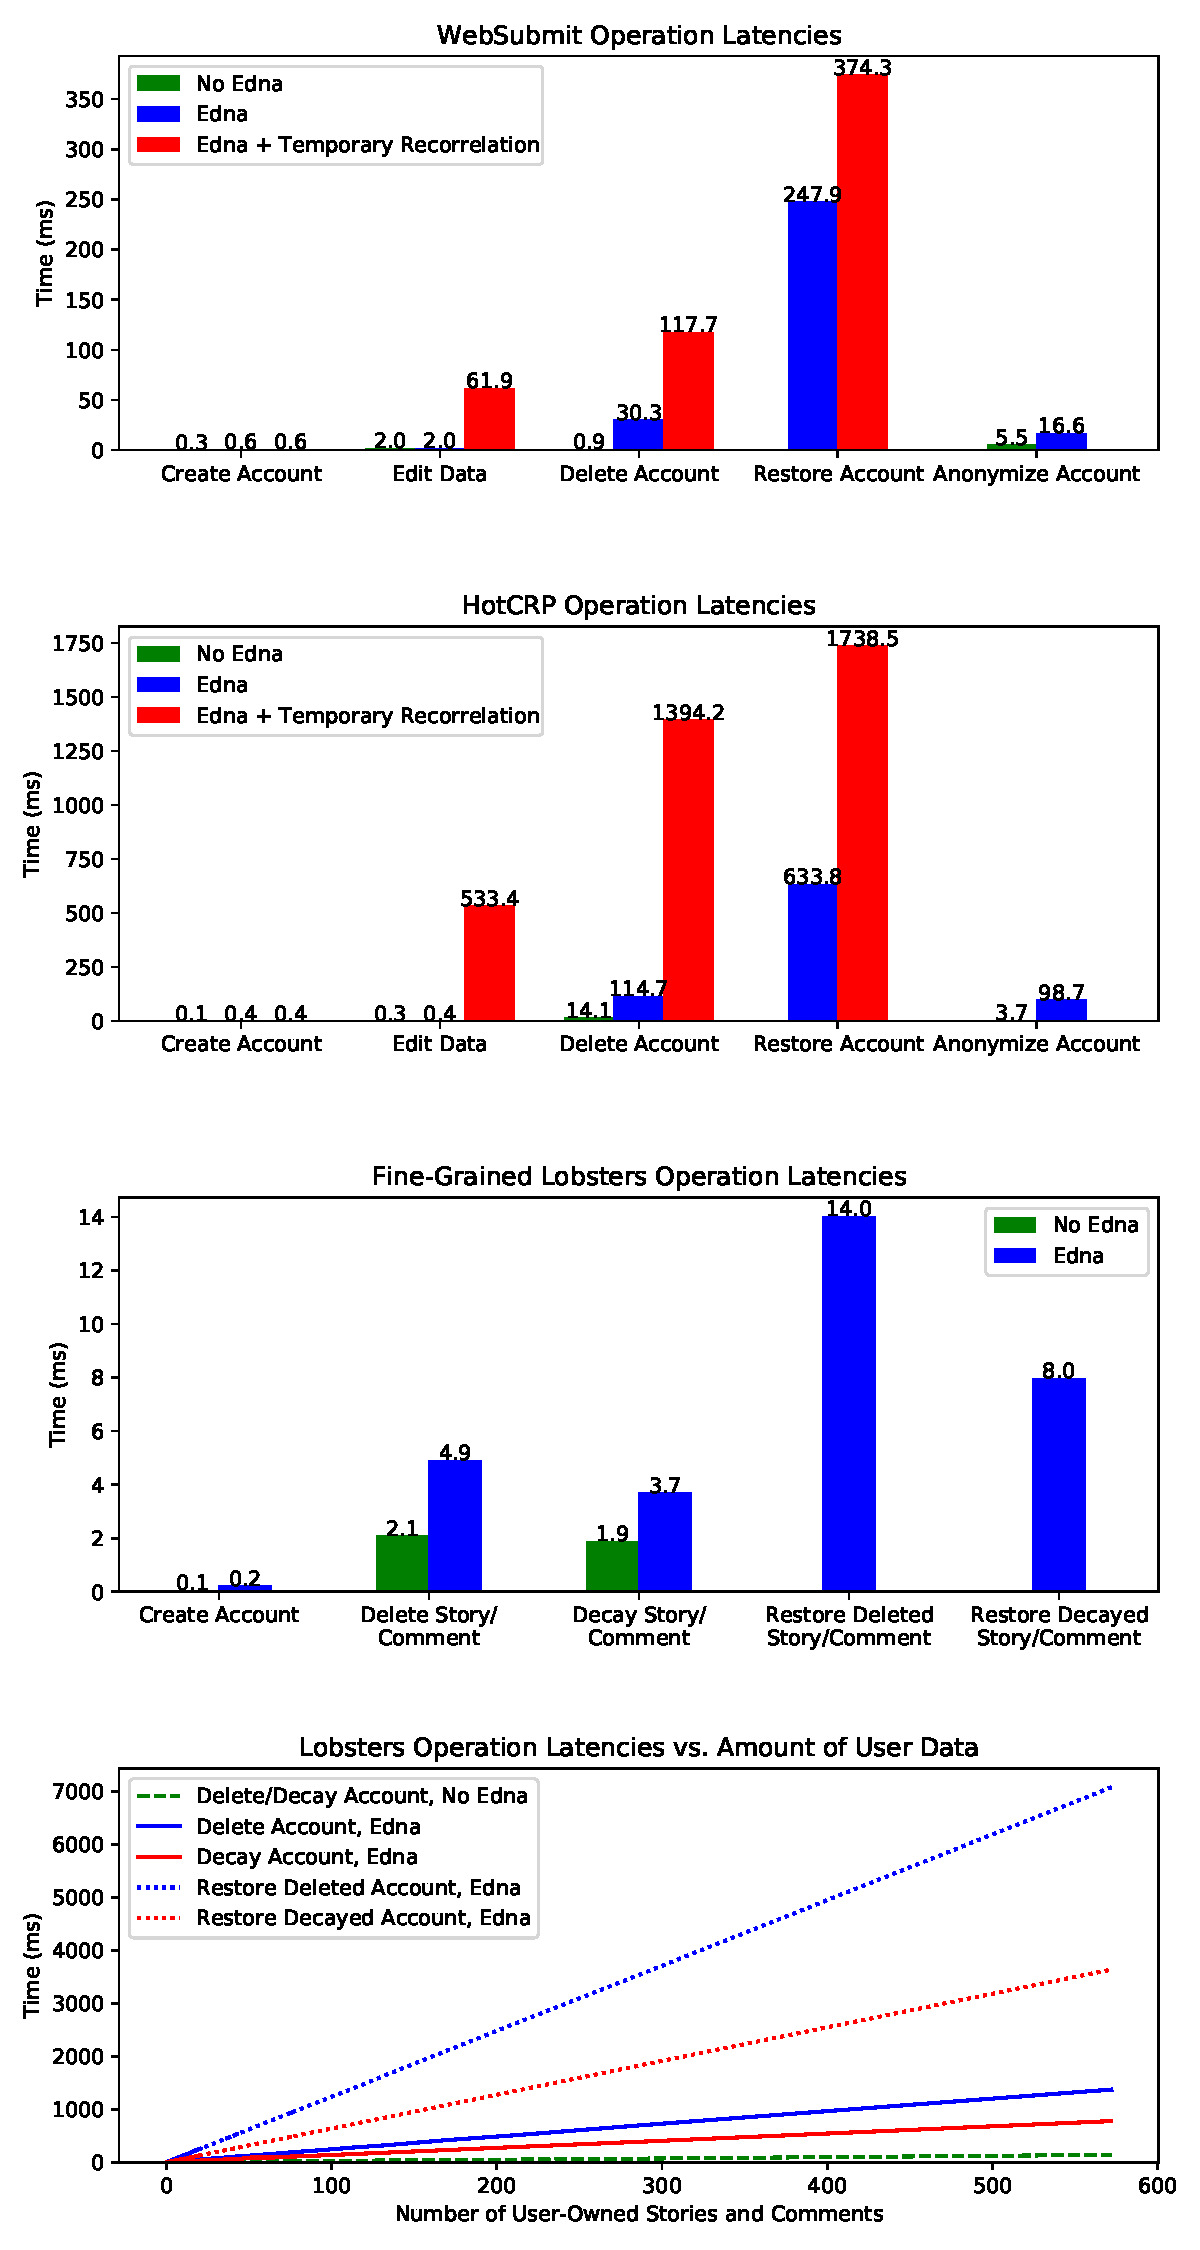
\includegraphics[width=0.5\textwidth]{figs/client_op_stats}
    \caption{Latencies of disguise-related actions when implemented manually by the
    application developer without \sys, and with \sys.
    Each bar shows the median latency; ranges indicate the 5th to 95th
    percentile latencies.  }
    \label{fig:client_opstats}
\end{figure}

\begin{table*}[h!]
\begin{center}
\begin{tabular}{ c c }
\textbf{DB Op} & \textbf{Time (ms)}\\
\hline
Update DB Row & 0.1\\
Select DB Rows & 0.2\\
Remove DB Rows & 0.2\\
Reveal Deleted Row (DB Select + Insert) & 0.2 \\
Create + Register Principal & 0.1\\
\end{tabular}
\quad
\begin{tabular}{ c c }
\textbf{Crypto Op} & \textbf{Time (ms)}\\
\hline
Generate Keypair & 301\\
Encrypt SpeaksFor Record & 0.4\\
Decrypt SpeaksFor Record & 3.0\\
Encrypt Diff Record & 0.3\\
Decrypt Diff Record & 3.0\\
\end{tabular}
\end{center}
\caption{Amount of time required to run different operations required to apply and reveal disguises.}
\label{tab:opstats}
\end{table*}

%
Figure~\ref{fig:client_opstats} shows the median cost across user accounts of performing disguise-related actions with and
without \sys, and with record batching enabled in \sys.
Note that \sys enables editing of anonymized data and account restoration. Thus, we have no
comparable baseline latency without \sys for editing anonymized data or account restoration.
Record batching also has no effect in creating user accounts and editing unanonymized data (as no
records are involved).

\sys-WebSubmit and \sys-HotCRP support the same disguise-related operations, namely
account creation, deletion/restoration, anonymization, and editing anonymized data.
\sys-Lobsters supports account creation and deletion/restoration as well, but has account decay (and
subsequent restoration) instead of account anonymization.  It does not support editing anonymized
data (accounts can be restored in order to edit decorrelated data). In these benchmarks, we measure
the cost of GDPR-compliant account deletion and restoration.

\sys-WebSubmit users all have approximately the same amount of data (a set number of answers to
lecture questions). Thus, the spread in latencies is low. The simplicity of \sys-WebSubmit's
disguises---which touch at maximum two database tables---lead to fairly low latencies even for
expensive operations such as restoring deleted accounts (250ms).

\sys-HotCRP reviewers have slightly more variable amounts of data \lyt{TODO?} depending on the
assignment of papers to reviewers. \sys-HotCRP's disguises are far more complex than
\sys-WebSubmit's, touching 12 tables, and performing a mix of deletions and
decorrelations, leading to higher median latencies in general, even for the baseline.

\sys-Lobsters users' amount of data follows a skewed distribution, with most of the 5000 users
having fewer than 10 stories and comments, and a handful of users having over 300 stories and
comments. \sys-Lobster supports more complex disguises than \sys-WebSubmit and \sys-HotCRP,
touching 15 tables, and performing a mix of deletions, decorrelations, and modifications. This leads
to a higher latency as the amount of user data grows comparable to that of users in \sys-HotCRP and
\sys-WebSubmit.

In general, using \sys without record batching increases the latency of
disguising and revealing accounts. Latency-critical tasks such as editing (unanonymized) data or
creating an account are largely unaffected by \sys. With record batching, we observe drastic
improvements in the latencies of account disguising and revealing, and in edits of anonymized data.
%
To explain these costs, we break them down into fine-grained operations shown in
Table~\ref{tab:opstats}: every disguise action requires some DB operations and,
if using \sys, may require cryptographic operations.

\textbf{Creating an account} with or without \sys performs a database insert. Using \sys additionally
requires registering the new user as a principal, which assigns the user a (pre-generated)
private-public key pair, stores metadata about the new principal's key in \sys's storage, and
returns the corresponding private key to the application.
Using \sys thus incurs only the cost of an extra database operation, since the high cost of key
generation is taken offline.

\textbf{Editing data} with or without \sys simply performs database updates. Editing anonymized
data, however, requires \sys to decrypt (with the client-provided decryption capability) \emph{all}
speaks-for records at the client-provided locator until it finds a speaks-for record linking the
client to the currently-owning pseudoprincipal.  For example, if anonymization of a user account
generates 20 speaks-for record ciphertexts at the same locator, then editing anonymized data may
perform up to 20 decryptions to determine which pseudoprincipals the client can act for.  Record
batching drastically decreases this cost by performing only one decryption to decrypt all speaks-for
records for a particular client and disguise.

\textbf{Account deletion or data decay} with or without \sys performs the same database operations
to remove, modify, or anonymize data. \sys incurs increased costs by additionally encrypting and
inserting one diff record for each deleted or modified object, and one speaks-for record for each
anonymized object.  With record batching, encryption occurs once per account, rather than once per
object.

\textbf{Account restoration} is only possible with \sys. \sys decrypts a record for each
piece of modified/removed/anonymized data, and performs database checks to ensure the data can be restored
(\eg that the corresponding lecture of an answer to reinsert still exists). If the checks pass
(which they do in this benchmark), \sys restores the data stored in the diffs.
Record batching drastically decreases this cost by performing only one decryption to decrypt all
records to restore.

\textbf{Anonymization} with or without \sys generates one pseudoprincipal per object to anonymize
(\eg answers for lectures in WebSubmit, or reviews in HotCRP). Anonymization selects the relevant answers
to anonymize, generates new pseudoprincipals, and performs DB queries to insert new pseudoprincipals
and to update objects to point to these new pseudopricipals (\eg updating foreign keys).
\sys incurs increased costs by additionally generating per-pseudoprincipal speaks-for records, and
encrypting and storing these speaks-for records with the appropriate public keys.
With record batching, encryption occurs once per account, rather than once per object.

\begin{table*}[t!]
\begin{center}
\begin{tabular}{ c | c c }
& \multicolumn{2}{c}{\textbf{Prior Applied Disguises}} \\
    \textbf{Op} & None & Anonymization \\
\hline
WebSubmit Delete & 30 & 112 \\
WebSubmit Restore & 250 & 372\\
HotCRP Delete & 114 & 1612 \\
HotCRP Restore & 629 & 1856 \\
\end{tabular}
\quad
\begin{tabular}{ c | c c }
 & \multicolumn{2}{c}{\textbf{Prior Applied Disguises}} \\
    \textbf{Op w/Batching} & None & Anonymization \\
\hline
WebSubmit Delete  & 3 & 30 \\
WebSubmit Restore  & 18 & 86\\
HotCRP Delete  & 51 & 880 \\
HotCRP Restore  & 73 & 998
\end{tabular}
\end{center}
\caption{Account delete and restore latencies before anonymization, and composed after anonymization.}
\label{tab:composition}
\end{table*}

\textbf{Composing Deletion After Anonymization.}
\lyt{TODO}
Account deletion post-anonymization requires \sys to perform temporary recorrelation find data of
pseudoprincipals that the user is authorized to remove along with their account. \sys incurs latency
increases from decrypting all speaks-for records of the user, and from performing the deletion or
modification queries for each discovered pseudoprincipal (in addition to the original user).

Account restoration may also restore pseudoprincipal-associated data, which requires temporary
recorrelation to access to pseudoprincipal-associated records produced from the account deletion.
\sys thus additionally decrypt speaks-for records for all pseudoprincipals of the user, which causes
the the increase in latency.\lyt{Numbers?}

%%%%%%%%%%%%%%%%%%%%%%%%%%%%%%%%%%%%%%%%%%%%%%%%%%%%%%%%%%%%%%%%%%%%%%%%
\subsection{Resource Use}
\label{s:eval-res}

Each generated pseudoprincipal adds an additional row to the users table in WebSubmit; \sys also
stores public-key metadata for each principal (and pseudoprincipal), and (in-memory) encrypted
ciphertexts for records.  Clients keep track of capabilities and locators that are emailed to them in
the form of URLs that allow for account restoration or post-anonymization editing.

%%%%%%%%%%%%%%%%%%%%%%%%%%%%%%%%%%%%%%%%%%%%%%%%%%%%%%%%%%%%%%%%%%%%%%%%
\subsection{Impact on Normal Application Use}
\label{s:eval-conc}

\begin{figure*}[t!]
    \centering
        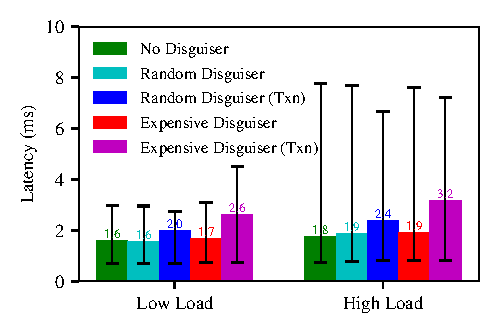
\includegraphics[width=0.45\textwidth]{figs/lobsters_concurrent_results}
        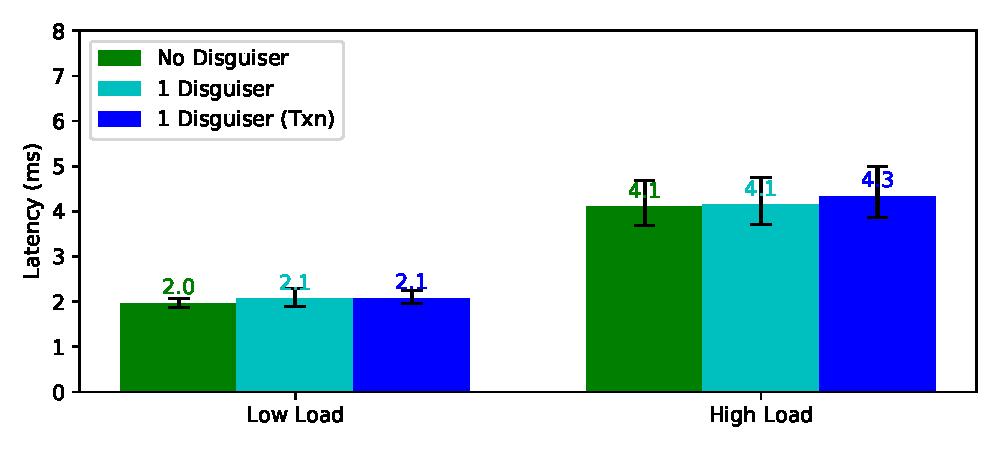
\includegraphics[width=0.45\textwidth]{figs/websubmit_concurrent_results}
    \caption{Impact of disguising (account deletion and revealing) on 100 users concurrently running
    normal application answer edits. We show the median latency; ranges indicate the 5th to 95th
    percentile latencies.    
    \textbf{Left (Lobsters)} TODO.
    \textbf{Right (WebSubmit)} tests with an adversarial,
    write-only user workload of edits that modify the same table.
    }
    \label{fig:concurrent}
\end{figure*}

Figure~\ref{fig:concurrent} shows the impact of concurrently-running disguise actions on the latency
of normal application operations.

We first test the impact of disguising in \sys-Lobsters. We first achieve ~80\% CPU load by running
30 threads that model production Lobsters traffic. These threads simulate performing different
Lobsters operations (\eg loading the front-page, posting stories) according to measured access
frequencies and popularity distributions in production\lyt{CITE}. In this workload, 85\% of all
operations are front-page loads, which fetching stories and vote counts.

An additional number of threads simulate disguising users: these users (in the worst-case) decide to
simultaneously delete their account (\eg in response to some social media campaign). At some later
point in time, these users decide to come back and (in the worst case) simultaneously restore their
accounts.
We observe that even when the number of disguisers increases to 100, the latency of normal Lobsters
operation remains unaffected.

We then test an adversarial, write-only workload with WebSubmit. As a baseline, we achieve ~60\% CPU
load by running 100 threads that each continuously edit a user's lecture answers with 250-500ms
pauses between edits. This write-heavy workload achieves particularly high contention because all
edit queries modify the same database table; MySQL uses table-level locking for \texttt{MEMORY}
tables.

We then add an additional number of threads to simulate simultaneously disguising users.  While
fewer than 16 users disguising themselves at once has minimal impact on edit latency, 30 users doing
so causes spikes up to 4000ms.  These spikes come in pairs, with the larger second spike in the pair
coinciding with concurrent revealing (and the first of the pair coinciding with disguising);
revealing has greater impact due to its higher latency and compute costs.
%
Record batching improves these results by reducing the load generated by disguise actions: latency
spikes decrease to under 1500ms.

While we focus on normal application operation latency, we note that
disguise operation latency increases proportional to the overall system load (\eg due to MySQL’s
table-level locking). But this is acceptable, as disguises aren't time critical; in practice, they
still complete within a few seconds even at 60-80\% system load.
%
What matters is that normal application requests have acceptably low latency even in the presence of
disguising, which we achieve under realistic workloads (largely reads, with queries dispersed among
tables). If the workload becomes adversarial, \sys can prevent normal operation latency spikes by
rate-limiting disguise actions.
